\section{Tools}

\section{Simulation Design}

Figure \ref{fig:simulation_design} shows the general simulation setup that is used to test the software components of the proposed system.

\begin{figure}[h]
	\centering
		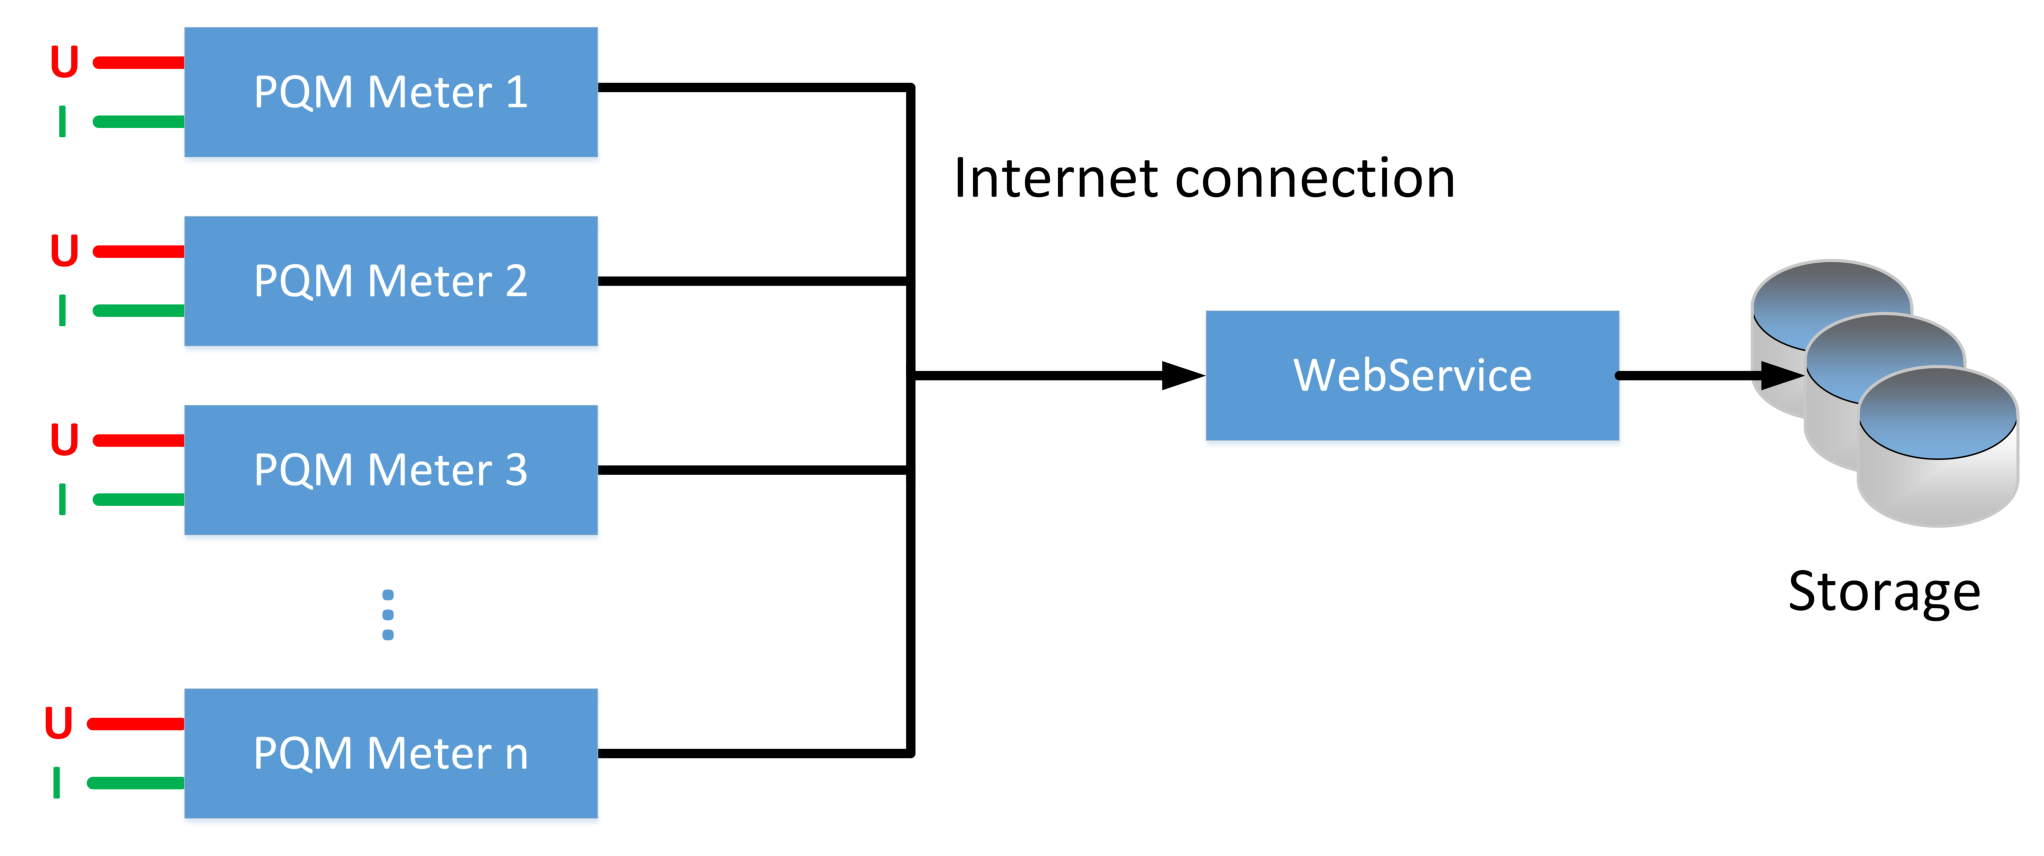
\includegraphics[scale=0.4]{graphics/simulation.eps}
	\caption{Simulation design}
	\label{fig:simulation_design}
\end{figure}

Different parameters of the simulation can be changed, such that different environments can be simulated and evaluated against each other. The following enumeration describes the parameters that can be adapted as input data to the simulation:

\begin{itemize}
	\item Bandwidth of the Internet connection
		\subitem Wired connection: 100 MB/s, 50 MB/s, 20 MB/s, 10 MB/s
		\subitem WiFi connection: 
		\subitem Cellphone connection: LTE (), 4G (), 2G (), GPRS ()
	\item Number of PQM meters
	\item Number of Webservices
	\item Transmitted data
		\subitem Raw data
		\subitem Preprocessed data
  \item Storage
		\subitem File archive
		\subitem SQL database (MySQL)
		\subitem NoSQL database (CrateDB)
\end{itemize}

\section{Evaluation}

\section{Impact on System Design}